\documentclass[12pt]{handout}

\author{Jim Fowler}
\course{Math 1181H}
\date{Autumn 2012}

\usepackage{nopageno}
\usepackage{tikz}
\usepackage{amsmath}

\usetikzlibrary{calc}
\usetikzlibrary{through,positioning}
\usetikzlibrary{arrows}

\DeclareMathOperator{\CAT}{CAT}

\setlength{\parskip}{1.5ex}
\setlength{\parindent}{0in}
\geometry{margin=0.3in}
\usetikzlibrary{patterns}

\title{Log-Log graph paper}

\long\def\symbolfootnote[#1]#2{\begingroup%
\def\thefootnote{\fnsymbol{footnote}}\footnote[#1]{#2}\endgroup}

\begin{document}
\maketitle

\textbf{Congratulations!}  Here is some log-log graph
paper\symbolfootnote[1]{By the way, let $f(n) = $ the number of hits when you
  search for the number $n$ on the internet; you should try plotting
  $f$ on log-log paper sometime.  The result is very entertaining.}
for you to plot the Dehn function.

\vfill

\begin{center}
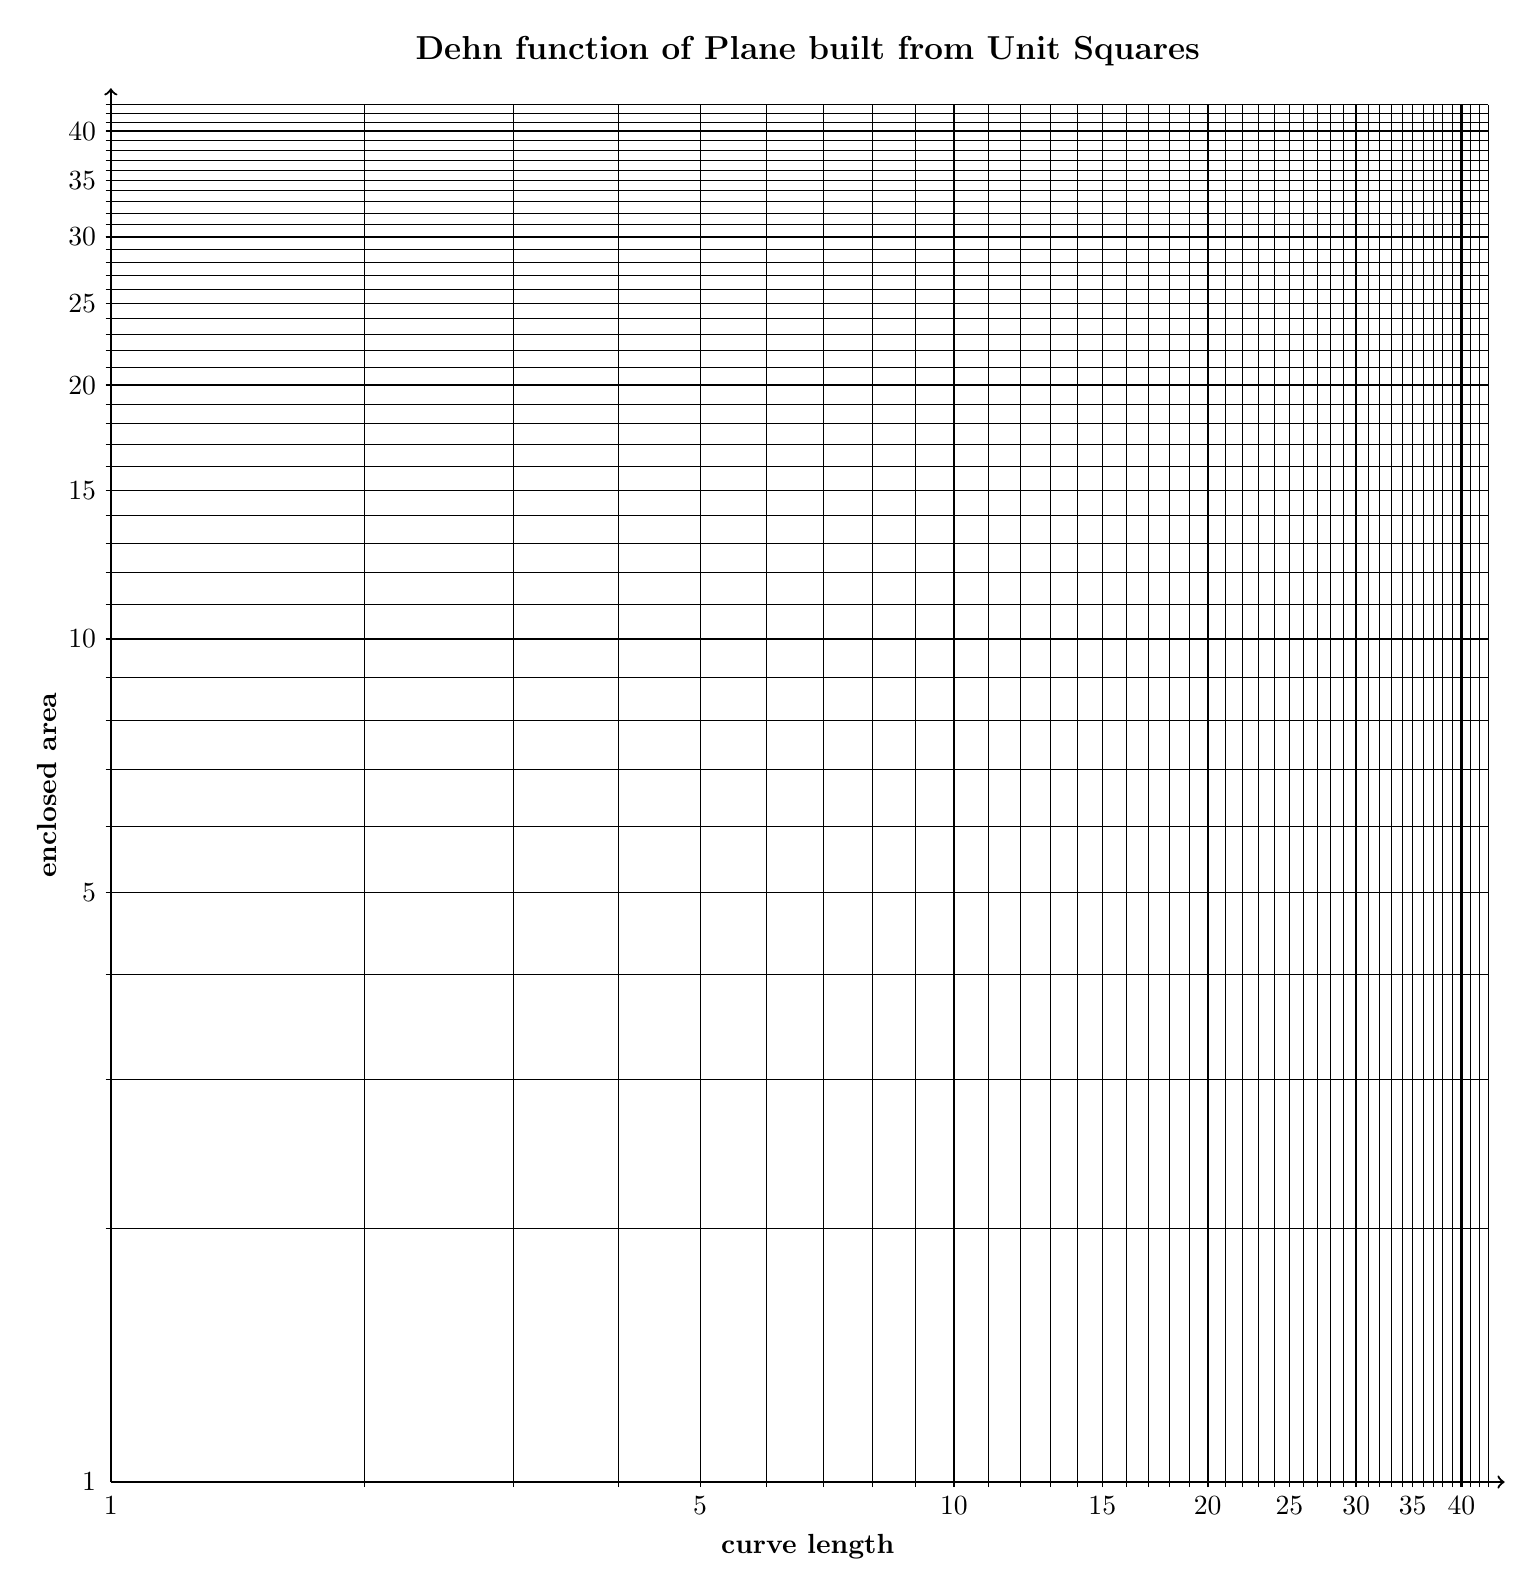
\begin{tikzpicture}[scale=4.65]
    \draw[thick,->] (0,0) -- ({ln(45)},0);
    \draw[thick,->] (0,0) -- (0,{ln(45)});

    \foreach \x in {2,...,43}
    \draw[line width=0.3pt] (-0.4pt,{ln(\x)}) -- ({ln(43)},{ln(\x)});
    \foreach \x in {2,...,43}
    \draw[line width=0.3pt] ({ln(\x)},-0.4pt) -- ({ln(\x)},{ln(43)});

    \foreach \x in {10,20,30,40}
    \draw[thick] (-0.4pt,{ln(\x)}) -- ({ln(43)},{ln(\x)});
    \foreach \x in {10,20,30,40}
    \draw[thick] ({ln(\x)},-0.4pt) -- ({ln(\x)},{ln(43)});

    \foreach \x in {1,5,10,15,20,25,30,35,40}
    \node[anchor=east] (label) at (-0.4pt,{ln(\x)}) {\x};
    \foreach \x in {1,5,10,15,20,25,30,35,40}
    \node[anchor=north] (label) at ({ln(\x)},-0.4pt) {\x};

    \node[anchor=center] (x axis) at ({ln(45)/2},{ln(45)+0.1}) {\large
      \textbf{Dehn function of Plane built from Unit Squares}};

    \node[anchor=center] (x axis) at ({ln(45)/2},-5pt) {\textbf{curve
        length}};
    \node[anchor=center,rotate=90] (x axis) at (-5pt,{ln(45)/2})
    {\textbf{enclosed area}};

  \end{tikzpicture}
\end{center}
\vfill


\end{document}

%%% Local Variables: 
%%% mode: latex
%%% TeX-master: t
%%% End: 
